\documentclass[../main.tex]{subfiles}

\begin{document}
	
We have implemented a total of 5 methods for conducting inference on the continuous time state space model described by \autoref{eq:2__1__our_state_space_model}. 

\begin{enumerate}
	\item A generic one-dimensional bootstrap particle filter (PF) which inferred only the returns ($x_2$) state.
	\item A drift-corrected bootstrap particle filter which infers both price ($x_1$) and returns ($x_2$) states simultaneously. 
	\item A Rao-Blackwellized Particle Filter (RBPF) for the case of a symmetrical \asd ($\beta = 0$)
	\item Dense Sampling improvement for the RBPF to reduce sample impoverishment 
	\item Adaptive Sampling improvement for the RBPF to create a fully adapted RBPF 
\end{enumerate} 

In this section, we will compare and discuss the results obtained by the 5 inference algorithms. Unless explicitly stated, simulated data (with the simulation process described in \tofix{Secion X}) has been used to obtain the results in this section. This provides us with both ground truth data for the states, as well as the actual parameters used, allowing us to test the effectiveness of the inference algorithms without the complications of parameter inference.

As a brief comparison of all the 5 inference algorithms, Figure \ref{fig:4__1__comparison} shows the performance of all 5 inference algorithms using a large number of particles ($N=10000$).

\begin{figure}[h!]
	\centering
	\subfloat[Root Mean Square Error (RMSE) of the price($x_1$) process \label{fig:4__1__comparison_price}]{
		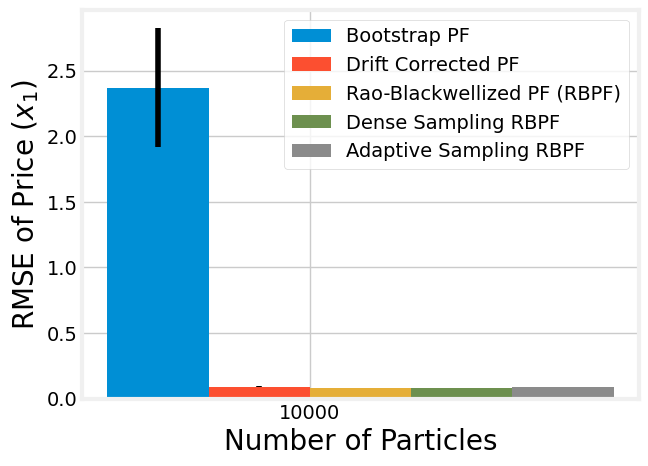
\includegraphics[height=4.5cm]{../plots/4__1__comparison_price.png}}
	\qquad
	\subfloat[Root Mean Square Error (RMSE) of the returns($x_2$) process  \label{fig:4__1__comparison_returns}]{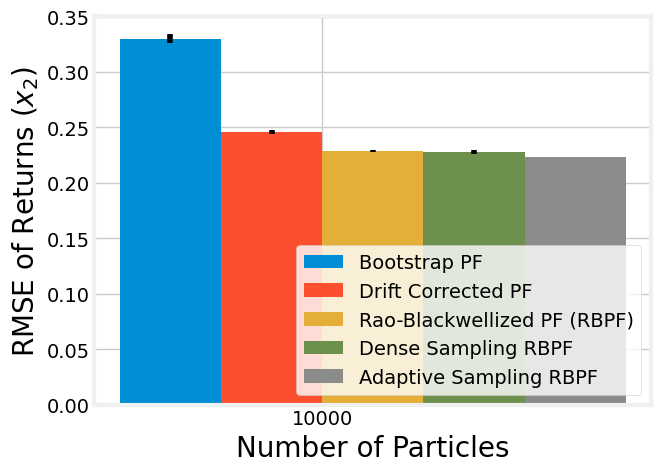
\includegraphics[height=4.5cm]{../plots/4__1__comparison_returns.png}}
	\caption{Comparison of all inference algorithms, $N = 10000$ particles}
	\label{fig:4__1__comparison}
\end{figure}
	
We can conceptually divide the 2 inference algorithms into 2 classes: generic particle filtering based inference and rao-blackwellized particle filtering based inference. We will compare and discuss these 2 classes of inference algorithms separately in the next 2 subsections.
	
\end{document}